% ===============================================================
%
% For tracking purposes - this is V2.0 - May 2012

\documentclass{sig-alternate}
\usepackage{float}
\floatstyle{boxed}
\newfloat{pseudocode}{h}{lop} %{chapter}
\floatname{pseudocode}{\textbf{Algorithm}}
\usepackage{amsfonts}
\usepackage{amsmath}
%\usepackage{amsthm}
\usepackage{amstext}
\usepackage{amssymb}
\usepackage{algorithmic}
\usepackage{fainekos-macros}  
\usepackage{amsbsy}
\usepackage{graphicx}
\usepackage{todonotes}
%\usepackage{geometry}
%\usepackage{latexsym}
%\usepackage{makeidx}
\usepackage{enumerate}      
%\usepackage{url}
%\usepackage{rotating}
%\usepackage[labelfont=bf,textfont={sl,bf},lofdepth,lotdepth]{subfig}
\usepackage{fixltx2e}
%\usepackage{ifthen} 
%\usepackage{bigdelim,multirow,xspace}
%\newtheorem*{IEEEproof}{Proof}
%********************************************************************
\graphicspath{{figures/}}

\newcommand{\agentInstanceSet}{A}
\newcommand{\agentTypeSet}{\Ac}
\newcommand{\scenarioSet}{\Sc}

\begin{document}
%
% --- Author Metadata here ---
\conferenceinfo{EMSOFT}{2015 Amsterdam, The Netherlands}
%\CopyrightYear{2007} % Allows default copyright year (20XX) to be over-ridden - IF NEED BE.
%\crdata{0-12345-67-8/90/01}  % Allows default copyright data (0-89791-88-6/97/05) to be over-ridden - IF NEED BE.
% --- End of Author Metadata ---

%\title{When all you have is not a hammer: multi-formalism verification of autonomous plans}
\title{When you have more than one hammer: multi-formalism verification of autonomous plans}
\date{\today}
% Just remember to make sure that the TOTAL number of authors
% is the number that will appear on the first page PLUS the
% number that will appear in the \additionalauthors section.

\maketitle

\begin{abstract}
%Autonomous and semi-autonomous systems are now an accepted part of the economy and society, whether they are autonomous robots in shipping warehouses or autonomous appliance robots in the home.
%The success of these robots can be attributed, in part, to the fact that either they function in highly controlled environments where their interactions with other agents are structured, or their tasks are simple enough to accommodate unstructured and unpredictable environments.
%In this paper, we develop a framework for formally verifying the safety of autonomous systems operating in unstructured environments in the presence of other unpredictable agents. 
%Using autonomous vehicles as a running example, 
%we present a decomposition of an autonomous system's mission into scenarios and agents, and a rich representation of these two elements in terms of hierarchical communicating hybrid automata. 
%Our goal is to formally verify that the behavior of the autonomous system is safe in a given scenario, which possibly involves other unpredictable (nondeterministic) agents.
%Therefore, we include in our framework a translator from this rich representation into the formalisms of various formal verification tools, to enable the use of the most appropriate tool for a given verification task. 
%The fact that multiple tools are needed is illustrated with the verification of the safety of a lane change maneuver, which requires the use of a timed automaton verification tool, and a rechability tool.
%Another goal is to allow control engineers to use these formal tools as part of their design process. 
%Therefore, we develop a scenario authoring tool, and a domain-specific language with formal semantics, for enabling rapid prototyping and verification of controllers' designs.
%


\end{abstract}

% A category with the (minimum) three required fields
\category{H.4}{Information Systems Applications}{Miscellaneous}
%A category including the fourth, optional field follows...
\category{D.2.8}{Software Engineering}{Metrics}[complexity measures, performance measures]

\terms{Theory}

\keywords{ACM proceedings, \LaTeX, text tagging}
\section{outline}
\label{outline}
\todo[inline]{this section will be removed from final paper, of course}
Introduction
\begin{itemize}
	\item The benefits of autonomous systems.
	
	\item The acceptance of autonomous systems in the economy and our daily lives.
	
	\item Autonomous vehicles as a running example. What are the "real-world" challenges? (e.g. lane change in some detail, then just list others like pedestrians, other drivers,etc)
	
	\item What are the technical challenges facing the development of autonomous vehicles? (e.g. properties with priorities)
	
	\item How are these challenges addressed in today's technology and literature?
	
	\item What remains to be done?
	
	\item Which piece of the puzzle are we addressing in this paper? Illustrate with the running example of a lane change maneuver.
	
	\item How are we addressing it?
	
	\item The need for formal methods.
\end{itemize}



Modeling framework
\begin{itemize}
	\item Scenarios and agents (don't dwell too long on this, just need to mention that we are verifying one scenario in this paper, but we have a plan for how this fits with overall mission verification)
	
	\item HCHA: because we need a representation rich enough to express on it different types of properties, which apply to different components of the complex autonomous vehicle
	
	\item Specification languages: should be suited to the verification goal. Here, reachability and LTL

\end{itemize}

Lane change in the formalisms.
\begin{itemize}	
	\item Formal model of lane change in terms of HCHA for system, LTL for scenario goal, and reach sets for safety. Controller is a discrete controller in grid world.
	
	\item Lane change requirements can be verified with timed automata, so need to translate HCHA. Give translation.
	
	\item How results are mapped back to HCHA
	
\end{itemize}


Experiment
\begin{itemize}
	\item Experimental setup: simulation or actual little vehicles? UPPAAL, dReach, make it available online
	
	\item results
	
\end{itemize}

Future work
\begin{itemize}
	\item Tool chain: from design entry to formal DSL (implementing HCHA) to design files for relevant tools
	\item priority of requirements?
\end{itemize}

\section{Introduction}
\label{introduction}

{\it Autonomy from human intervention in the machines that surround us promises many benefits.}

{\it Because of these benefits, autonomous and semi-autonomous systems are now an accepted part of the economy and the household.}

{\it Autonomous vehicles are a particularly challenging class of autonomous systems.}

{\it On a typical trip, the autonomous vehicle must recognize, enter, complete and exit many scenarios in a safe and timely manner. Example scenarios include traffic lights, roundabouts, pedestrians, weather conditions, etc. 
It is not known, ahead of time, what the specific sequence of encountered scenarios will be.}

{\it The corresponding technical challenges can be broadly divided into two categories: operation in a highly unpredictable environment, and a task (navigation) that must be executed at many levels of abstraction.}

{\it The environment of the autonomous vehicle is unpredictable: will others obey the laws, what will traffic conditions be, etc? What is the vehicle's objective in the short run?}

{\it There is also a wide separation between the highest levels of plan execution ("go from A to B") and the lowest levels of plan execution ("accelerate steadily for the next 5 seconds"). How do we guarantee consistency between the commands at the different levels?}

{\it The safety of the car's passengers and of the people in its immediate environment is imperative at all times. 
	What does safety mean in a given scenario?
	In an emergency, how do we recognize what laws can be broken to preserve safety?}

\todo[inline]{Safety,comfort,performance}
%\footnote{Interesting legal question: if the car, by design, violates some law to avoid harming someone, how long before the manufacturer gets sued for purposefully breaking the law? Think about swerving too hard and "losing control of the vehicle" to avoid running over someone.}
%\footnote{Other notions of safety, such as passive safety where the autonomous system must not endanger others via \emph{inaction}, or extensions of the safety imperative to not damaging property (and not just people) are not covered here. We note nonetheless that guaranteeing that the active safety imperative is obeyed contributes to guaranteeing these other notions are also obeyed.}
%For people to feel comfortable interacting with potentially dangerous autonomous agents, like autonomous cars, it is imperative that they be confident that these systems are at least as safe as the human-operated systems they are replacing.
%In fact, for there to be an economic value behind the introduction of autonomous systems, they must, among other things, guarantee an increased level of safety relative to the current system. 
%Increased and more consistent efficiency and effectiveness at completing their tasks are other desiderata, which are outside the scope of this paper.
%We call this the `dorasical' environment, from the Greek $\delta \rho \acute{\alpha} \sigma \eta$ for action.


{\it Guaranteeing safety to a socially acceptable degree requires formal guarantees.}

{\it Today we have theories that deal with high-level planning in a discrete grid world: where the car should go given where everyone else is.}

{\it We also have discrete theories for verification of temporal logic properties of the closed-loop system modeled as a Kripke structure. Some of these theories are amenable to model checking.}

{\it Control theory provides analysis and design tools of low level controllers. Automatic analysis tools exist but are limited in scope.}

{\it Because of the large degree of unpredictability, compute- and memory-intensive low level methods can't be used alone (let alone manual methods). Yet because of the safety imperative, we can't rely on non-guaranteed abstractions.  In this paper, we demonstrate the need for using multiple formalisms in the verification of autonomous plans. We illustrate this with a case study of a typical lane change maneuver.}

\begin{exmp}[Lane change maneuver]
	
	Throughout this work we will take as a case study the following example. At various instances we will zoom in on on specific scenarios within the sequence of events. The case study shows a target vehicle driving on a two lane road network that includes a merge which introduces another vehicle into the path of the target vehicle. The target vehicle's planning system may autonomously decide to initiate a lane change manuever to get around the other vehicle. The scenario terminates with an intersection governed by a traffic light. This scenario contains two vehicle agents (with different plans, 1 traffic control (infrastructure agent), and 1 road network. 
	
	\todo[inline]{who's involved in this scenario; what is the goal of ego vehicle; what is the sfaety constraint; why model checking alone won't suffice.}
\end{exmp}

From a planning perspective we define the safety of the discrete controller of the target vehicle to be the satisfaction of the following safety and liveness properties:
\begin{enumerate}
	\item The target vehicle may not exceed the speed limit (safety).
	\item The target vehicle may not collide with any other vehicles (if they exist) on the road (safety).
	\item The target vehicle must stop at a red light (safety).
	\item The target vehicle must eventually complete the scenario (liveness).
It is clearly possible to specify these properties using LTL operators (always and eventually).
\end{enumerate}

%Work on autonomous navigation: DARPA urban challenge papers, controller synthesis papers.
%
%DSL: that paper by the french authors, others?
%
%Scenarios and agents: there has to be a tonne here...the papers referenced by Matt in the APEX preso
%
%Interaction between model checkers and other verif tools: CEGAR, matthias and CMU guy, spaceex.
%
%Other semi-formal verif: staliro, breach, apx bisimulations.

\subsection{Notation}
We denote the set of integers including 0 with $\Ne$. 
Given a subset $S$ of the reals, $S^* = S \setminus \{0\}$ and $S_+ = S \cap [0,\infty)$,
while $S_+^* = S \cap (0,\infty)$.
\section{The modeling of autonomous plans}
\label{framework}

\begin{itemize}
	\item Scenarios and agents (don't dwell too long on this, just need to mention that we are verifying one scenario in this paper, but we have a plan for how this fits with overall mission verification)
	
	\item HCHA: because we need a representation rich enough to express on it different types of properties, which apply to different components of the complex autonomous vehicle
	
	\item Specification languages: should be suited to the verification goal. Here, reachability and LTL
	
\end{itemize}

\subsection{Decomposing a mission into scenarios and agents}
\label{scenarios and agents}
To motivate our thinking about the problem of safe autonomous navigation, we consider the case of a trip between two designated points.
On such a trip, the autonomous car will face a number of situations, or \emph{scenarios}, which it must know how to recognize, enter, negotiate, and exit in a safe and timely manner.
For example, the car will encounter roundabouts, 
traffic lights and four-way intersections, 
on-ramps to highways, 
lane changes, 
pedestrians,  
and various traffic signals like speed limits, school zones, etc.
We therefore think of a driving mission as an \emph{ordered sequence of scenarios}.
The exact sequence that will be encountered is not known ahead of time. 
%For example, it is not known whether some road has a large pothole that must be avoided.
Moreover, it is clear that some scenarios, like traffic lights, will be encountered more than once, albeit with minor site-specific differences. 
The key observation however is that the diversity of scenarios is, to a first order of approximation, finite. 
That is, there is a recognizable, finite set of scenario \emph{types} that is sufficient to describe most autonomous navigation missions.
The remaining variability among scenarios can be parametrized: e.g., the number of cars at a roundabout, or the current speed limit.

To formally define a scenario, we first outline its elements.
First, within each scenario, we can recognize a recurring set of entities: 
the autonomous vehicle whose operation we seek to verify (a.k.a. the \emph{ego} vehicle), the other vehicles on the road, pedestrians, traffic signage, and the road network itself. 
We will refer to these as \emph{agents}: an agent is an entity that functions continuously and autonomously in the environment, and whose presence can be sensed by other agents. 
\todo[inline]{main literature for agents}
Formally, we recognize the following set of four agent \emph{types}, whose semantics are given in the next section.
\[\agentTypeSet = \{\texttt{vehicle, pedestrian, road, trafficSignage}\}\]
Each agent type can have many (parametrized) instances, e.g. $\texttt{trafficSignage}$ can have instances speedLimit(70mph), speedLimit(25mph), HOVLane(3pm-6pm).
We denote the set of instances of agents in $\agentTypeSet$ by $I(\agentTypeSet)$.
Clearly, $I(\agentTypeSet)$ is infinite.
When we just speak of an agent, we mean an agent instance.

Formally, we define a scenario instance as follows. 
The elements of a scenario will be formally defined in the following sections.
\begin{defn}[Scenario instance]
	A scenario instance is a tuple $(\agentInstanceSet,\behavior, \lawSet, \Phi, Init, \exitConditions)$ where
\begin{itemize}
	\item $A$ is a collection of agent \emph{instances} from the set $I(\agentTypeSet)$.
	The set $\agentInstanceSet$ always includes the ego vehicle, i.e., the system whose behavior we want to verify.
	%
	\item $\behavior = \{\behavior_a \sut a \in \agentInstanceSet \setminus \{egoVehicle\}\}$ is a bounded-time behavior description for each of the other agent instances.
	Describing the behavior $\behavior_a$ of an agent instance requires us to formally describe an agent. 
	We do so in Section \ref{HCHA}.
	What assumptions we make on the behavior of other vehicles is captured in $\behavior$.
	%
	\item $\lawSet = \{l_0,\ldots,l_p\}$ is a finite set of $p \in \Ne$ traffic laws. 
	A law $l_i$ is a temporal logic formula indicating how the law constrains the behavior of the ego vehicle, but not the other agents. 
	I.e. it is a specification on the ego vehicle that must be satisfied. 
	% 
	\item $\Phi$ is a set of goals that must be met by the ego vehicle while in this scenario. 
	Now $\Phi$ and $\lawSet$ may both be expressed as (temporal) logic specifications on the system's behavior and therefore may be grouped together as one set.
	However it helps to keep these two aspects of the scenario separate: 
	that laws are constraints on the vehicle's behavior, and scenario goals are objectives to be met.
	%
	\item $Init$ is an initialization of the scenario, which defines a valid initial set of states for the agents when the scenario starts. $Init$ is formally defined in the next section.
	% 
	\item $\exitConditions$ is a set of condition describing how and when the scenario ends.
	The conditions are described as temporal logic formulae with atomic propositions on the states of the agents in the scenario.
	The formulae are required to be satisfiable by finite prefixes.
	That is, for any formula $\formula \in \exitConditions$, if there exists a trace $\sttraj$ of the system that satisfies $\formula$, then there exists a finite prefix of $\sttraj$ that satisfies $\formula$.
\end{itemize}
Let $\Sc = \{s_0,s_1,\ldots,s_{N-1}\}$ be a set of scenario instances. 
Then \textbf{a mission} $M$ is a finite string on $\Sc$, $M \in \Sc^*$.
\end{defn}

\todo[inline]{mission as an automaton?}

The logic in which a law $l_i$ or exit condition $\formula_i$ is expressed will depend on the formalism used to model the scenario's agents. 
We will have more to say about this in the following sections.

Because a mission is a sequence of scenarios, if we can verify the safety of the autonomous system's behavior in each scenario,
and compose the scenarios in a safe manner, 
then we have verified that the mission is safe.
In the rest of this paper we formalize the correct composition of scenarios and illustrate it with a case study in Section \ref{caseStudy}.
Note that in this paper, we do not study how to \emph{generate} missions for verification. 
Rather we assume that we are given mission to be verified. 
The problem of mission generation and verification coverage will be the subject of future research.

\begin{prob}[Correct composition of scenarios]
	
	\end{prob}


\begin{exmp}[Lane change continued]
	The mission can be decomposed into the following scenarios:
	$M = $ DriveStraight, ChangeLane, PassOnTheLeft, StopAtFourWayIntersection.
	Each of these scenarios contains two instances $v_{ego}$ and $v_2$ of the \texttt{vehicle} agent type, one \texttt{road} agent instance, no \texttt{pedestrian}s and one \texttt{trafficSignage} agent.
	The behavior $\behavior_{v_2}$ is given by a sequence of reach sets as detailed in Section \ref{otherAgents};
	briefly, $\behavior_{v_2}$ gives the area occupied by $v_2$ at any moment in time.
	An example applicable law, expressed in discrete time LTL, is $l \defeq \always(position_{ego} = a \implies X position_{ego} \geq a)$, to indicate that backing up is not allowed.
	Note that LTL is not ideally suited for this requirement since we need one formula per speed threshold $a$. A more concise logic (e.g., TPTL \cite{alur94_really}) would allow us to directly say $l \defeq \always(position_{ego}(t+1) \geq position_{ego}(t))$, while still being reasonably computationally tractable.
		
	There are two exit conditions for the DriveStraight scenario: either the ego vehicle reaches the end of the current road segment (i.e. , it reaches the intersection). 
	Or, it gets too close to the leading vehicle $v_2$, in which case it must exit and scenario ChangeLane begins.
	The $Init$ set for ChangeLane is the union of two sets $Init_1$ and $Init_2$.
	$Init_1$ is the set of 2D positions on the road where $v_ego$ is behind $v_2$ and within some distance $d_{min}$ of $v_2$.
	$Init_2$ is the set of 2D positions of $v_{ego}$ that are some distance $d_{turn}$-close to the intersection.
	I.e., we consider the lane change to be provoked by excessive proximity to the leading vehicle $v_2$, or by proximity to the intersection.	
\end{exmp}

It should be noted that the initialization of a scenario may have a mission-dependent part, like $Init_2$ in the example.
This highlights the need to do verification \emph{in the context of the mission}, as the context provides information on what needs to be verified.
	
%	E.g an instance of scenario $s_0$ (Roundabout) might have the agents 
%	\begin{eqnarray*}
%		\agentInstanceSet = \{&egoVehicle, otherVehicle1, rndAbt(3), \\ 
%		& speedLimit(25mph)\} \subset I(\agentTypeSet)
%	\end{eqnarray*}
%	where $egoVehicle$ and $otherVehicle1$ are instances of type $\texttt{vehicle}$, 
%	$rndAbout(n)$ is an instance of $\texttt{road}$ indicating a round-about with $n$ entry points (which are also exit points),
%	and $speedLimit(Vmph)$ is an intance of $\texttt{trafficSignage}$ indicating a speed limit sign that reads $V$ mph.
%	Another scenario instance has the agents
%	\begin{eqnarray*}
%		\agentInstanceSet = \{&EgoVehicle, OtherVehicle1, rndAbt(2), \\ 
%		& speedLimit(35mph)\} \subset I(\agentTypeSet)
%	\end{eqnarray*}
%	

\subsection{Hierarchical communicating hybrid \\automata}
\label{HCHA}
Because autonomous systems are physical systems controlled by software, hybrid automata (HA) are a suitable formalism for modeling them.
Because the complexity of autonomous systems is significant, they are typically designed at multiple levels of abstraction, 
with different teams handling the design at different levels.
E.g. the mapping team might design the algorithm for finding the waypoints along a shortest route from start to end.
For this design, knowledge about, say, the powertrain control of the car is immaterial and abstracted away.
Indeed, details about the road itself are abstracted away as well.
Instead, it is represented as a directed graph.

The resulting system's description is given at multiple levels of abstraction (or multiple levels of detail). 
To model this situation, we adopt \emph{hierarchical} HA: each mode of the HA is itself an HA, down to some level.

Finally because these HHA, each representing an agent, are sensed by other agents in the scenario, we must model this sensing. 
We do so via the inputs to each HHA: given agent instance $a$, every other agent is associated with an input port on $a$.
When that other agent is within sensing distance of $a$, that input port is occupied by that agent's sensed information.


\todo[inline]{Refer to Charon}


\subsection{What is safety?}
\label{safety}

For people to feel comfortable interacting with potentially dangerous autonomous agents, like autonomous cars, it is imperative that they be confident that these systems are at least as safe as the human-operated systems they are replacing.
In fact, for there to be an economic value behind the introduction of autonomous systems, they must, among other things, guarantee an increased level of safety relative to the current system. 
Increased and more consistent efficiency and effectiveness at completing their tasks are other desiderata, which are outside the scope of this paper.

In this section, we formalize the safety imperative: 
that is, what it means for an autonomous system to be safe, in the context of autonomous vehicles.
\todo[inline]{lit review on safety}
The general (active) safety imperative is that the autonomous car must not take actions that directly endanger the car's passengers (including the driver) or people in the environment that is susceptible to its actions.
We call this the `dorasical' environment, from the Greek $\delta \rho \acute{\alpha} \sigma \eta$ for action.
\footnote{Other notions of safety, such as passive safety where the autonomous system must not endanger others via \emph{inaction}, or extensions of the safety imperative to not damaging property (and not just people) are not covered here. We note nonetheless that guaranteeing that the active safety imperative is obeyed contributes to guaranteeing these other notions are also obeyed.}

For an autonomous vehicle, this safety requirement means not colliding with other agents in the environment (cars, pedestrians, and traffic signage), or entering unsafe regions of the environment, like opposing traffic lanes or obstacles.
This holds regardless of the scenario type the ego vehicle is engaged in. 
But specializing this imperative to a given scenario type allows us to break it down into more specific requirements which, when formally expressed, can facilitate the model checking task.
Intuitively, by specifying certain ways in which safety can be violated, we guide the model checker towards finding those ways, in effect constraining the search space.
\todo[inline]{cite XOR (formalize => prove)? (in that order)}
These scenario-appropriate properties are then expressed in a formal logic like Linear Temporal Logic (LTL) \cite{Pnueli77sfcs} or Metric Temporal Logic (MTL) \cite{Koymans90}, and formally verified on the formal model of the scenario.
To avoid confusing common terminology, we will call these \emph{safety-inducing properties}, because when we write them as logic formulae they don't take the form of what is usually referred to as a safety formula. 
That is, they are not in the form $\always (x \notin \text{Unsafe set})$.
But once they are satisfied, they guarantee, by construction, that the safety imperative is satisfied in this scenario.
\todo[inline]{Future: Can we take the absolute safety mandates and automatically specialize them to scenarios? I.e. given the set of state trajectories of the car, automatically derive, from the scenario, some constraints that constrain the search for the subset of trajectories that end in harming someone in that particular scenario?}
\todo[inline]{safety algebara?}
 
\section{Verifying the safety of abstract plans for discrete maneuvers}
\label{verifyingSafety}

\todo [inline ] {Do we really mean the first sentence. Lets again talk about the difference between correctness and safety tomorrow. I think correctness equals goal satisfaction, safety equals dont crash}
{\it To verify the lane change scenario given in the previous sections, we must integrate two formalisms: timed automata for correctness of the controller's actions, and reachability for safety of the controller's actions.} 
We have already defined the basic representation of an autonomous driving scenario as a HCHA. 
A single mode of the HCHA can be viewed from two perspectives: discrete as represented by a state in a timed automaton, and continuous as represented by a plant and systems of nonlinear ODEs. 
Interaction between these representations occurs when guard conditions in the discrete representation are encountered. 
One way of reasoning about the goal specifying behavior of the scenario controller is to investigate the safety and performance of the timed automaton using model checking methods.

{\it Thus, we translate the scenarios's HCHA to timed automata.} Given the HCHA it is possible to create a map which has abstracts the system to a timed automaton on which we can perform verification tasks. 
\begin{thm}
	Let \(X\) and \(Y\) be vector fields on \(M\) and \(N\) respectively and let \(\phi: M \rightarrow N\) be a smooth surjective map. Then vector field \(Y\) is an abstraction of vector field \(X\) with respect to \(\phi\) iff for every integral curve \(c\) of \(X\), \(\phi \circ c\) is an integral curve of \(Y\). \cite{Pappas1998} 
\end{thm}
If we consider that the abstraction of the system is overapproximate, then we may conclude that it is sufficient to check safety properties on the abstraction \cite{Pappas1998}. A result that returns safe must be safe. However, given a counterexample to a proposition specifying a safety property one cannot be sure that it is not spurious. Thus, it would also be natural to attempt to refine abstraction to remove any spurious counter examples. We will address this notion of counterexample guided abstraction refinement shortly \cite{Clarke2003}, but first it is essential to discuss the hierarchical aspect of the HCHA.

Hierarchical controls are commonly used to reason about systems which control realistic levels of complexity. Thus, the scenario controller as implemented in the real system will interact with the motion planner. When considering the motion planning controller, reachability is the formalism for which it is convenient to explore the feasibility and safety of the planned trajectories. Reachability analysis determines safety by checking the intersection of reachable sets of the underlying dynamics with unsafe regions. This investigation leads to the fundamental question:{\it if the discrete controller is safe, and the motion planner is safe, is the hierarchical composition of the two safe?} Fortunately, the answer to this question can be yes. 

\begin{prop}
	Let \(X_1\), \(X_2\), \(X_3\) be vector fields on manifolds \(M_1\), \(M_2\), and \(M_3\) respectively. If \(X_2\) is an abstraction of \(X_1\) with respect to the map \(\phi_1 : M_1 \rightarrow M_2\) and \(X_3\) is an abstraction of \(X_2\) with respect to map \(\phi_2 : M_2 \rightarrow M_3\) then \(X_3\) is an abstraction of \(X_1\) with respect to abstracting map \(\phi_1 \circ \phi_2\) \cite{Pappas1998}
\end{prop}

{\it Thus, once each subsystem can be verified, we must map back the verification results to the HCHA formalism.}
Going a step beyond the results in \cite{Pappas1998} We propose that the relationship between verification, in the sense of logical analysis of a system, and control, in the sense of the evolution of state variables described by nonlinear ODEs, is so tightly intertwined that new approaches to system design are necessary. By viewing the activities of correct by construction controller design and verification as tightly coupled processes instead of distinct options we can design solutions for richer, more complex problems. Returning to the lane change case study, we briefly summarize state of the art work in the area.

One approach to designing safe lane change and evasive vehicle maneuvers explores the use of reachability to generate an automaton which switches between motion primitives in an offline phase. Online the precomputed reachable sets of motion primitives are compared to the reachable sets of the other agents. It is possible to perform the reachable set calculations online because there is less non-determinism about the initial state of the other agents, there is no tracking controller in the loop, and the dynamics are simpler.\cite{Hess2014}

Another approach explores the use of reachability entirely online as a means of verifying and controlling vehicle maneuvers. In order to ease restrictions on computation timing linearized vehicle dynamics are used when considering the target vehicle. Perturbations representing external conditions such as road surface quality and sensor noise are added in order to improve the accuracy of the linearized model. Current run times are on the order of 4-5 seconds making this approach impractical for unexpected events. Furthermore the linearization requires the overapproximation of the system making the results conservative.\cite{Althoff2014b}

Notions of reachability have also been used within the CEGAR framework introduced by Clarke et al. The CEGAR framework for automatic refinement of system abstractions checks to see whether counterexamples generated during model checking of an abstraction of the system of interest are real by examining  whether the counterexample is spurious on a less abstract version of the system. Through this process the abstract version of the system can be iteratively refined.\cite{Clarke2003}

The CEGAR framework can be extended as an alternative to the online reachability analysis presented by Althoff and Hess. Through the combination of correct by construction controller synthesis with approximate solutions to constrained reachability problems feasible trajectories are computed for nonlinear systems. While the authors present a solution to the motion-planning problem for nonlinear systems, they do not consider other dynamic agents. Furthermore, the authors' decision procedure is not complete. Finally, the presented method of refining the control automaton relies on enumerating and ranking solutions under a cost function which is not well defined in their work.\cite{Wolff2013}

In our problem we consider several other vehicles in the environment with simple 2-D kinematics and the target vehicle with the nonlinear bicycle model dynamics. While in general the reachability problem for non-linear hybrid systems is undecidable. Recent work has shown that if a user is able to specify a bound on the ODE which is an arbitrary positive rational number \(\delta\), then propositions in first order logic over a region \textit{unsafe} can be evaluated \cite{gao2014delta}. Specifically a system, \(H\), is \(safe\) if it cannot reach \(unsafe\), and \(H\) is \(\delta-unsafe\) if \(H^d\) can reach \(unsafe\). 

The unsafe region of a driving scenario as the intersection between the reachable set of the target vehicle and the reachable set of the other vehicles in the scenario over a specified time horizon \(\Delta t\). We note that using the concept of \(\delta-reachability\) does not have any affect on the quality of our results when compared with traditional approaches to reachability. If the system is safe then a logical proof is generated showing that the original system \(H\) cannot reach the unsafe region. Alternately if the \(\delta-reachability\) analysis returns unsafe then the answer means that an overapproximated version of the system, \(H^{\delta}\) reaches the unsafe region. Clearly, one can adjust \(\delta\) so as to discover the robustness of the system. 

\todo [inline] {Houssam: add information about sampling-based motion planning techniques.} 
\todo [inline]{Matt: add in something about Sarah Loos' work on thm proving}

\todo[inline]{literature review}

\todo[inline]{Pending the lit review, might be worth investigating two approaches we discussed:
if the boxes of the partition used by controller are over-approximations of the reach set alphabet, and model checker returns SAT, then must compute reachability for every satisfying trace. Obviously, can get expensive.

Else, we can partition the state space using the reach set alphabet as explained on the board, so the model checker's answer needn't be concretized: by construction it gives a sound and complete answer.

I'd be very surprised if these two don't have antecedents in the literature, they're natural enough...

Because ours is a verification task, it's not up to us to dictate the controller's view of the world.
}

\section{Case study}
\label{caseStudy}
\subsection{Scenario Description}
Passing manuever is scenario on 2 lane road, target vehicle, 1 environmental vehicle.
\subsection{Target Vehicle Model}
\begin{enumerate}
	\item Target vehicle has non linear dynamics described by bicycle model.
	\item Trajectories are defined for right to left lane switch and left to right lane switch.
	\item Hybrid system modes are described by drive forward and lane change.
	\begin{enumerate}
		\item Lane change is hierarchical and has sub-modes, right to left, straight, and left to right.
		\item Each submode has same dynamics but implements a different motion primitive.
	\end{enumerate}
\end{enumerate}
\subsection{Environmental Vehicle Model}
Environmental vehicle has simple 2D dynamics, no specific controller, non-determinism describes state evolution.
\begin{enumerate}
	\item Environmental vehicle must drive forwards.
	\item Environmental vehicle must not change lanes if other lane is occupied.
	\item At every step the environmental vehicle can apply +/- some specified level of acceleration.
	\item At every step environmental vehicle can switch lanes if condition 2 is not violated.
\end{enumerate}
\subsection{dReal Model}
\begin{enumerate}
	\item 1 or 2 modes depending on lane change or passing.
	\item Dynamics are non linear bicycle model (insert figure)
	\item Plant controller is tracking controller which follows trajectory.
\end{enumerate}
\subsection{Controller with Partial Dynamics}
A finite transition system describing the passing manuever is given in UPPAAL (or NuSMV).
\section{Conclusions}
\label{conclusions}
{\it Autonomous plan verification presents two major challenges: a high level of unpredictability of the autonomous system's environment, and system execution that spans many levels of abstraction.}

{\it In this paper, we proposed a multi-formalism approach to verification to address these challenges, and illustrated it on a lane change scenario.}

{\it We also advocated a scenario verification framework.}

{\it In future work, we will automate the modeling and translation procedures, to allow the use of formal plan verification methods by control and system engineers.}

{\it We will also address the issue of prioritizing requirements in a given scenario to deal with emergencies.}
% Scenario authoring tool, DSL, tool bus
%\section{Design entry and the tool bus}
\label{designEntryAndToolBus}

\subsection{The tool bus}
\label{tool bus}
One of our goals in APEX is to formally verify the safety of the autonomous system's operation in all scenario types.
As we saw in Section \ref{safety}, the imperative to be safe is expressed by different logic properties in the different scenarios types.
To verify these properties, we must first decide on the appropriate formalism(s) in whic to express them (e.g. LTL, CTL, or MTL?) 
and the corresponding formalism for describing the autonomous system under verificaiton.
Secondly, we must decide on which tool to run to verify the property.
In general, we may expect that different properties, and different levels of abstraction at which they are verified, will require (or be better verified) using different formalisms and tools. 
For example, verifying a property of the continuous-time dynamics may be done using {\staliro}~\cite{AnnapureddyLFS11tacas},
whereas verifying a property of the discrete mission planner may be best done using UPPAAL \cite{BehrmannDLHPYH06qest}.
This motivates the creation of a translator from our detailed HCHA representation of the scenario instance to the different formalisms that are deemed useful. 
For example: timed automata, weighted timed automata, Ordinary Differential Equation (ODEs), impulsive systems,...etc.
See Fig.~\ref{fig:toolbus}.

\begin{figure}[tb]
	\centering
		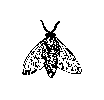
\includegraphics{figures/fly.eps}
	\label{fig:toolbus}
	\caption{The APEX tool bus.}
\end{figure}

The representation of a scenario and its agents in some Intermediate Representation (IR) allows the translation into many other formalisms.
The key requirement is that the IR must be at least as detailed as any target formalism.
Formally, we say that a model $\Mc_1$ (in formalism $F_1$, e.g. HCHA) is at least as detailed as model $\Mc_2$ (in formalism $F_2$, e.g. timed automata) if the behavior of $\Mc_2$ contains the behavior of $\Mc_1$: 
\[\behavior_{\Mc_1} \subset \behavior_{\Mc_2}\]
This is the familiar notion of behavior inclusion, and it is one more reason for choosing HCHA as the IR:
the most detailed analysis that can be made on the autonomous system is at the level of the continuous dynamics.
These are captured in the HCHA. 
Other aspects are also captured in the HCHA, as explained in Section \ref{HCHA}.
These details can be abstracted when translating the HCHA to a timed automaton to perform verification using UPPAAL.
On the other hand, had we chosen timed automata as our IR, we would not have been able to recover the true dynamics from the timed automaton's differential inclusions. This would preclude us from performing accurate reachability computations for example.

\todo[inline]{a word on jhow to transfer verif results back to HCHA}

APEX includes a tool bus: once a combination of tools is decided on for a particular verification task, the IR is translated to the formats of these tools and transmitted to them.

\subsection{Simulation model}
\label{simulation model}
Control engineers, who will be one of the main group of users of APEX, are mostly used to \emph{simulating} their designs under certain initial conditions and inputs from the environment to determine correctness. 
Simulation is also a quick way to get a qualitiative idea of what the system does, and is used iteratively to improve the design.
It is therefore important for APEX to provide a translation from the IR to a simulation tool, in addition to the translation to formal tools. 
We chose to add the MathWorks' Simulink \copyright to the tool bus.
Simulink is well-known to most engineers and has the advantage of a Graphical User Interface which can be leveraged as a design entry tool (see Section \ref{dsl}).

Note that because the simulation model will not be subjected to formal verification, there is no need to establish behavioral inclusion between its behavior and the IR.


\subsection{Scenario authoring tool and Domain-Specific Language}
\label{dsl}
How are the scenarios created? DSL and scenario authoring tool.


\bibliographystyle{abbrv}
\bibliography{emsoft15,conformance,HSCC2015_CompositionalConf,fainekos_bibrefs,houssam,SAREDnonlinear_2014}

%\balancecolumns

%\appendix
%\section{Headings in Appendices}

\end{document}
